\documentclass[11pt]{article}

\usepackage{natbib,unatbib}
\usepackage[nohide,twocolumn]{ulecnot}
%\usepackage{xyling}
\usepackage{tikz-qtree}
\usepackage{cancel}

\usepackage{ulogicproof}

\pagestyle{fancy}
\lhead{COGS 502 -- Programming and Logic}
\chead{Propositional Logic}
\rhead{Updated \it \today}
\lfoot{Umut \"Ozge}
\cfoot{}
\rfoot{Page \thepage/\pageref{LastPage}}
\setlength{\headheight}{13.6pt}

\begin{document}
\tableofcontents
\newpage
\section{Logic, language, thought}
\begin{itemize}
\item Be advised not to take logic as a model of human thought and reasoning.
\item Thought and reasoning are fairly complicated mental processes that do not
seem to behave as dictated -- at least -- by standard logics, and are the
subject of psychology, linguistics, artificial intelligence and
related fields. 

\item Laws of reasoning in logic, with some provisos, may be argued to apply to the end-products of thought,
idealized as propositions, predicates, quantification, and so on, which are
expressed in a formal (for now read as ``human-made'' or ``artificial'') language.
Logical laws can at best be utilized in justifying these end-products, rather
than characterizing how they are discovered or arise in the mind/brain of the
thinker.\footnote{See the introduction to \cite{reichenbach47} for some relevant
discussion. The classical work dealing mainly with the distinction between
human thought and inference on one hand and formal logic on the other is
\cite{johnsonlaird83}}
\item This distinction between discovery and justification starts to apply
already in mathematics before even approaching 	``everyday'' thinking. Theorems are
\textit{discovered} via largely intuitive (read as ``not scientifically explained
yet'') means, they are \textit{justified} (checked for validity) by formal tools
of logic.\footnote{Although the book itself is advanced for introductory level,
\cite[\S 16]{quine40} discusses this issue.}

\end{itemize}


\section{Syntax of Propositional Logic}
\label{induc}

\begin{itemize}
\item Any specification of a language starts with its alphabet.
\item[] Our alphabet for $L_0$ -- the name we will give to our language -- is made up of three sets:

\item[] Basic symbols:

\begin{align}
	P = \crbr{p,q,r,s,p_1,q_1,r_1,s_1,\ldots}
\end{align} 

\item[] Connective symbols:
 
\begin{align}
	C_1 &= \crbr{-} \\
 	C_2 &= \crbr{\land,\lor,\imp}
\end{align} 

\item[] Parentheses: \sysm{\crbr{(,)}}

\item We can also collect the parts of our alphabet under a single set:

\begin{align}
\Sigma = P \cup C_1 \cup C_2 \cup \crbr{(,)}
\end{align} 

\item Let's call an \uterm{expression}, any finite sequence of (possibly
repeated) elements from $\Sigma$. The following are some example expressions:

\[
p(\land r_{4291841}\lor-\quad\quad p-p \quad\quad   -))  \quad\quad \land\lor\land \quad\quad q_{345}\land
\]

\item It is not hard to see that there is no bound to the expressions we can
form this way. Call this non-finite set of all the possible finite expressions
formed by putting together a selection of symbols from $\Sigma$ in a specific
order $\Sigma^*$.

\item Usually, we are interested in expressions fulfilling certain
criteria -- a subset of the set of all possible expressions. We distinguish
these special expressions as the grammatical sentences of the language we are
interested in.  

\item Now we can define the grammatical expressions (sentences or \uterm{well-formed formulas})
of our language \sysm{L_0}. And we will see
that $L_0 \subset \sigmastar$.

\item As you might have already realized, we identify a language with the set of its grammatical sentences. 

\hrulefill
\begin{udefinition}{Well-formed formulas of \sysm{L_0}.}
\ezimeti{
\item[i.] \sysm{\alpha \in L_0}, if \sysm{\alpha \in P}.
\item[ii.] if $\alpha \in L_0$, so is $(\gamma\alpha)$, for $\gamma\in C_1$.
\item[iii.] if $\alpha$, $\beta \in L_0$, then so is $(\alpha\gamma\beta)$, for
$\gamma \in C_2$.
\item[iv.] Nothing else is in $L_0$.
}
\end{udefinition}
\hrulefill

\item An analytic procedure for defining the notion ``well-formed formula of $L_0$''. We
start from a complex expression and go down.

\hrulefill
\begin{udefinition}[wff's of $L_0$, ``top-down'']
\ezimeti{
\item[]
\item[i.]
$\alpha$ is a wff if $\alpha\in P$.
\item[ii.]  
$(-\alpha)$ is a wff iff $\alpha$ is a wff. 
\item[iii.]
$(\alpha\land\beta)$ is a wff iff $\alpha$ and $\beta$ are wff's. 
\item[iv.] 
$(\alpha\lor\beta)$ is a wff iff $\alpha$ and $\beta$ are wff's.
\item[v.]
Any expression that falls out of the above is not a wff.
}
\end{udefinition}
\hrulefill



\item Here is a synthetic way of specifying well-formed formulas. We start with the
simplest expressions and go up.

\hrulefill
\begin{udefinition}[$L_0$, ``bottom-up'']\label{defbot}
An expression is a wff (or belong to $L_0$)
iff it is built from the
elements of $P$ by applying a finite number of the following
operations:\footnote{What is the difference between the parentheses on the left
and right side of the equalities?}
\begin{align}
f_-(\alpha) & = (-\alpha)\\
f_\land(\alpha,\beta) & = (\alpha\land\beta)\\
f_\lor(\alpha,\beta) & = (\alpha\lor\beta)
\end{align}
\end{udefinition}
\hrulefill


\item This could be stated more formally:

 \hrulefill
 \begin{udefinition}[$L_0$, ``bottom-up'']
 An expression $\alpha$ is a wff iff there exists a sequence of expressions
 ordered in increasing length:

\[
 \alpha_1,\alpha_2,\ldots,\alpha_n
\]

such that \sysm{\alpha = \alpha_n}, and for any $\alpha_i$ for $i\leq n$, either
\ezimeti{
\item[i.] $\alpha_i \in P$;
\item[ii.] or there exists $j,k < i$ such that
$\alpha_i=f_\land(\alpha_j,\alpha_k)$ or $\alpha_i=f_\lor(\alpha_j,\alpha_k)$
\item[iii.] or there exists a $j < i$ such that $\alpha_i=f_-(\alpha_j)$,

where $f_-$, $f_\land$, and $f_\lor$ are as defined in
Definition~\ref{defbot}.
}
 \end{udefinition}
 \hrulefill

\item All these definitions not only define what the wff's of $L_0$ are, but
also their structure.

\item This is best observed over \uterm{derivation} (or construction) trees.

\begin{uexample}[Derivation trees]
Draw the derivation tree of \sysm{((p\land q)\lor((- r)\lor (q\land(- s))))}
\end{uexample}

\end{itemize}

\section{Semantics of Propositional Logic}

\begin{itemize}

\item In the previous section, we established the first half of a formal system.
We know which sequences of symbols constitute a well-formed expression of our
system. However, we do not yet know what those well-formed expressions mean. 

\end{itemize}

\subsection{Symbols}

\begin{itemize}
\item Signs and signification are central concepts in language, logic, and
computation.

\item An initial and rough conception of signification is a three-part
relation:\footnote{If you are interested in the study of signs, a good place
to start reading is the founders of the science of signs -- named
\uterm{semiotics} or \uterm{semiology}: Ferdinand de Saussure's ``Course
in General Linguistics'' and Charles Sanders Peirce' (pronounced like the
word \intx{purse}) ``Collected Papers''. Be warned that Peirce might be
quite challenging for beginners, but Saussure is a must read for everyone with a
serious interest in language.}

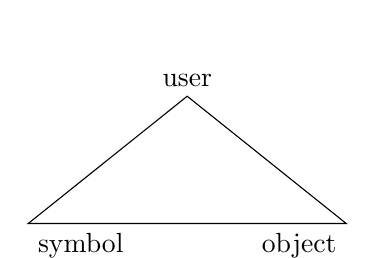
\begin{tikzpicture}[level distance=60pt]
\Tree [.user \edge[roof]; {symbol\hspace{50pt}object} ]
\end{tikzpicture}

\item Again some initial and rough characterizations: 
	\begin{itemize}
	\item A user uses a sign to \uterm{refer} to an object.
 	\item A sign \uterm{denotes} an object.
	\item A user has certain \uterm{intentions} about an object. 
	\end{itemize}
\end{itemize}


\subsection{Propositions}

\begin{itemize}
\item Let's characterize what a \uterm{proposition} is, indirectly  by way of 
natural language. Our characterization has two parts:
\begin{itemize}
\item[i.] Any expression that you can insert into the contexts ``\cntx\ is true'' or
``\cntx\ is false'' \textit{denotes} a proposition.\footnote{The contexts ``It is
the case that \cntx'' or ``It is not the case that \cntx'' will equally do,
barring some complications due to quotation. It gets yet more complicated when it comes to Turkish.
Can you see why?}
\item [ii.] There are no propositions that cannot be denoted as such.
\end{itemize}
	
The following expressions denote propositions:
	\begin{itemize}
	\item[]The earth revolves around the sun.
	\item[]D\"unya G\"une\c s etraf\i{}nda d\"on\"uyor.
	\item[]John likes Mary.
	\item[] If you multiply an even number with an odd number, you obtain an
	even number.
	\end{itemize}

while the following do not:
	\begin{itemize}
	\item[]Around the sun
	\item[]D\"unya G\"une\c s etraf\i{}nda d\"on\"uyor mu?
	\item[]Because John likes Mary
	\item[] If you multiply an even number with an odd number
	\end{itemize}

\item In other words, \uterm{declarative sentences} denote propositions.

\item Now let's assume that every proposition whatsoever has at least one
declarative sentence to express it.

\item From all we have above it follows that:

		Propositions are objects that can be (said to be) true or false.

\item Another way of saying this is that propositions are objects that have
\uterm{truth values}. 

% \item This much explication of what a proposition is will suffice for our
% purposes.


% \item Can you see what could be the problem with  equating declarative sentences
% with propositions?\footnote{Note to be read after discussing the question. For
% Willard van Orman Quine, one of the giants of analytical philosophy, what is
% problematic is not equating propositions with their linguistic expressions but
% rather the opposite. He objects to  maintaining that there are abstract objects
% called propositions which have their own life independent of the means that
% express or denote them. Here I chose the ``anti-Quinean'' exposition, because
% the discussion of Quine's objection is rather advanced for the current stage.
% See his ``Two dogmas of empiricism'' for a starter on this arguably the most
% central issue of analytical philosophy.}

\end{itemize}

\subsection{Propositional symbols}

\begin{itemize}

\item Propositional logic is called so, because its \uterm{atomic}\footnote{The
adjective \intx{atomic} serves to suggest that atomic symbols  cannot be broken
down to further components. This use of \intx{atomic} is a remnant from a
pre-nuclear conception of atoms.} symbols refer to objects called
\uterm{propositions}.

\item For instance, we can agree on things like, $p$ stands for the proposition
that the snow is white.  Given this, we can see that $p$ is interchangeable with
declarative sentences that express this proposition. Therefore, we can say 

\item[] $p$ is interchangeable with `The snow is white.'
\item[] $p$ is interchangeable with `Kar beyazd\i{r}.' 
\item[] and, so on.

\item Sometimes you will see `means', `abbreviates', `stands for', `equals to', `=', and so on, in place of
`is interchangeable with'.

\item When we use a basic symbol of $L_0$ as part of a well-formed formula of $L_0$, which
possibly consists of only that symbol, we assert the proposition referred
to by the symbol. So, 
\begin{align}\label{p}
p
\end{align}
says that the snow is white.

\item In science and other discourses, we are not only interested in
what propositions are expressed, but also whether the expressed propositions actually hold or not.

\item For any proposition whether it holds or not is indicated by its
\uterm{truth value}.\footnote{Note that we are counting on our intuitions here
for the meaning of ``holding'' \versus\ ``not holding''. A mathematical
rendition of this concept will follow soon.} If a proposition holds, we will say
that it is true, and its truth value is 1. If a proposition does not hold, we
will say that it is false, and its truth value is 0. Using the first two natural
numbers to designate truth values is totally arbitrary, you can pick any two symbols which will not lead
to confusion.

\item We will assume that, every proposition expressible in our system is either
true or false, there is no case in between.

\item A wff consisting only of a basic symbol of $L_0$ has the same truth
value as the proposition it expresses. Therefore, \xref{p} is true, or has the
truth value 1, if the snow is actually white, and is false, or has the truth
value 0, if it is not the case that snow is white.

\item From now on we will use ``formula'' in place of ``well-formed formula''
and directly speak of the truth or falsity of formulas of $L_0$.
\end{itemize}

\subsection{Valuations}

\begin{itemize}

\item A \uterm{valuation} is a function from the set of propositional symbols to
$\{ 0,1\}$. It tells which of our basic propositions are true and which are
false.

\item Assume we are dealing with a small subset of the language of propositional
logic, where we have only three propositional symbols $\crbr{p,q,r}$. Then there
are only eight possible valuations:
\begin{align}\label{valfunc}
\begin{array}[t]{c}
V_1 = \crbr{(p,1),(q,1),(r,1)} \\
V_2 = \crbr{(p,1),(q,1),(r,0)} \\
V_3 = \crbr{(p,1),(q,0),(r,1)} \\
V_4 = \crbr{(p,1),(q,0),(r,0)} \\
V_5 = \crbr{(p,0),(q,1),(r,1)} \\
V_6 = \crbr{(p,0),(q,1),(r,0)} \\
V_7 = \crbr{(p,0),(q,0),(r,1)} \\
V_8 = \crbr{(p,0),(q,0),(r,0)} 
\end{array}
\end{align}

\item These eight functions can be pictured also as a table:

\begin{align}\label{valtab}
\begin{array}[t]{c|c|c}
p & q & r \\
\hline 
1 & 1 &1 \\
1 & 1 & 0\\
1 & 0 &1 \\
1 &  0& 0\\
0 & 1 &1 \\
0 & 1 & 0\\
0 &  0& 1\\
0 &  0& 0
\end{array}
\end{align}

\item You can think of each function in \xref{valfunc} and, equivalently, each row
in \xref{valtab} designating a state of the world we are interested in. For
instance if you need to represent certain properties of a room for some reason and the
propositional symbols are associated with the following propositions,

\begin{align}
\begin{array}{ll}
p: & \text{lights are on}\\
q: & \text{the door is locked}\\
r: &\text{the room is occupied}
\end{array}
\end{align}


each valuation corresponds to a certain state of the room. States are
mutually exclusive, since at a given time the room is in exactly one of the possible states.

\end{itemize}

\subsection{Interpretation}

\begin{itemize}

\item To systematically characterize the meanings of formulas of propositional
logic, we will make use of an interpretation function $\mathcal{I}$ that takes a valuation and
a formula as input and gives a truth-value as output.

\item For atomic formulas, those comprising of a single propositional symbol,
defining the function is straightforward. 


\begin{udefinition}\label{isimple}

For any formula $P$ and a
valuation $V$,

\begin{align*}
\mathcal{I}(P,V) = V(P)\text{, if } P \text{ is atomic}. 
\end{align*}

\qed
\end{udefinition}

\item Given that $V$ is a function from propositional symbols to truth values
and $P$ is an atomic formula comprising of a single propositional symbol, $V(P)$
gives you the truth-value of the expressed proposition according to the given
valuation.

\end{itemize}

\subsection{Truth-functional connectives}

\subsubsection{Conjunction}

\begin{itemize}

\item As we saw above in defining the syntax of propositional logic, one way to
build complex formulas out of simple ones is
\uterm{conjunction}. On the meaning side, a conjunction asserts that both
conjuncts are true. If at least one of the conjuncts fails to be true, then the
conjunction fails to be true as well. If $p$ stands for snow's being white and
$q$ stands for Berlin being the capital of France, 
\begin{align}
(p \land q)
\end{align}
is true if and only if the snow is white and Berlin is the capital of France.

\item We can extend the definition of the interpretation function $\mathcal{I}$ as
follows: For any formulas $P$ and $Q$ and valuation $V$:


\begin{udefinition} \label{iconj}
\begin{align*}
\mathcal{I}((P\land Q),V) & = 1 \text{ if both } \mathcal{I}(P,V) = 1 \text{ and }
\mathcal{I}(Q,V) = 1\\ 
& = 0, \text{ otherwise}\nonumber
\end{align*}

\qed
\end{udefinition}

\item Note that the interpretation function $\mathcal{I}$ again takes two
arguments, a formula and a valuation, but this time we want the first argument
to be a conjunction.

\item It is also possible to take the conjunction itself as a function that maps
a pair of truth values to a truth value. The input pair is the truth-values of
the left and the right conjuncts, respectively. Such functions are called
\uterm{truth-functions}, as the value of the function depends entirely on the
input truth-values. The customary way to express truth-functions is a
\uterm{truth-table}: 

\begin{align}
\begin{array}{c|c|c}
P & Q & P \land Q \\ \hline
1 & 1 & 1\\
1 & 0 & 0\\
0 & 1 & 0\\
0 & 0 & 0
\end{array}
\end{align}

\item A more compact way to express the same function is as follows, where the first column
gives the values for the left conjunct and the first row gives the values for
the right conjunct:

\begin{align}
\begin{array}{c|cc}
\land & 1 & 0 \\ \hline
1 &1 &0 \\
0 &0 &0  
\end{array}
\end{align}

\hrulefill
\begin{uexample}\label{exconj1}
Given the formula $(p\land q)$ and the valuation $\crbr{(p,1),(q,0)}$,
\begin{align}
\mathcal{I}((p\land q), \crbr{(p,1),(q,0)}) = 0 
\end{align}
since $\mathcal{I}(p,\crbr{(p,1),(q,0)}) = 1$, but
$\mathcal{I}(q,\crbr{(p,1),(q,0)}) = 0$.

\qed
\end{uexample}
\hrulefill

\item As you might have noticed, in characterizing the interpretation function
$\mathcal{I}$ we are using capital symbols like $P$ instead of $p$. There is a
reason for this. The lower-case symbols like $p$, $q$ and so on are part of our
alphabet and are used to refer to atomic propositions. On the other hand the
upper-case symbols like $P$ are used and will be used to refer to arbitrary
formulas. An arbitrary formula can be of any complexity as well as being atomic.
If you go back to \xref{isimple} you will see that we started with $P$ but then
further restricted what $P$ can stand for by the expression `If $P$ is atomic'.

\hrulefill
\begin{uexample}\label{exconj2}
This time we are given a more complex formula $((p\land q)\land r)$ and the
valuation $V=\crbr{(p,1),(q,0),(r,1)}$,

As our formula to be interpreted is a conjunction at the top level, we need to
use the rule for conjunction given in \xref{iconj}. What we need to compute is
the value of 

\begin{align}\label{a0}
\mathcal{I}(((p\land q)\land r), V) 
\end{align}

which dictates that 
\begin{align}\label{a1}
\mathcal{I}((p\land q), V) 
\end{align}
and 
\begin{align}\label{a2}
\mathcal{I}(r, V) 
\end{align}
both be 1.

Further computations will reveal that while \xref{a2} is evaluated to 1,
\xref{a1} is evaluated to 0; therefore the value of \xref{a0} is 0. 

\qed
\end{uexample}
\hrulefill

\item As examples \xref{exconj1} and \xref{exconj2} show, in computing the
truth-value of a formula we need to use the notions `if', `both', and `and' borrowed from
natural language. It is possible and desirable to define the interpretation
function fully in mathematical form. Here is one way to do it: 

\begin{udefinition} \label{iconj2}
\begin{align*}
\mathcal{I}((P\land Q),V) & = \mathcal{I}(P,V) \times \mathcal{I}(Q,V) 
\end{align*}

\qed
\end{udefinition}

\item With definitions \xref{iconj2} and \xref{isimple} at hand, we can express
the computation involved in example \xref{exconj2} as follows:

\begin{align}
\mathcal{I}(((p\land q)\land r), V) & = \mathcal{I}((p\land q),V) \times \mathcal{I}(r, V)\\
                                    & = \mathcal{I}(p,V)\times \mathcal{I}(q, V)\times \mathcal{I}(r, V) \nonumber \\
									& = 1 \times 0 \times 1 \nonumber \\
									& = 0
\end{align}


\end{itemize}

\subsubsection{Disjunction}
\begin{itemize}

\item Another binary connective is \uterm{disjunction} (or
\uterm{alternation}).
It differs from conjunction in being more tolerant about falsehood. The
disjunction of two sentences come out true if at least one of the disjuncts is
true. With the same propositions being expressed by $p$ and $q$ as above,

\begin{align}
(p \lor q)
\end{align}

is true if and only if the snow is white, or Berlin is the capital of France,
\emph{or both}.


% \item Note that we use ``if and only if'' in stating the cases under which
% conjunction and disjunction are true. This is to say that they are false
% otherwise. 

\item Here is the truth-table for disjunction:

\begin{align}
\begin{array}{c|c|c}
P & Q & P \lor Q \\ \hline
1 & 1 & 1\\
1 & 0 & 1\\
0 & 1 & 1\\
0 & 0 & 0
\end{array}
\end{align}

and disjunction as a truth-function:

\begin{align}
\begin{array}{c|cc}
\lor & 1 & 0 \\ \hline
1 &1 &1 \\
0 &1 &0  
\end{array}
\end{align}

\item We add disjunction to the interpretation function as follows:

\begin{align}
\mathcal{I}((P\lor Q),V) = \mathcal{I}(P,V) + \mathcal{I}(Q,V) -
\mathcal{I}(P,V) \times \mathcal{I}(Q,V)
\end{align}


\end{itemize}

\subsubsection{Negation}

\begin{itemize}

\item Negation is a device that flips the truth-value of whichever formula it is
adjoined to.\footnote{Adjoining `$-$' and $P$ yields `$(-P)$' according to the
syntax we defined for $L_0$.} 

\item The interpretation function $\mathcal{I}$ handles negation as follows: For
any formula $P$ and valuation $V$,
\begin{align}
\mathcal{I}((-P),V) &= |\mathcal{I}(P,V) - 1|
\end{align}

\item The truth-table is,

\begin{align}
\begin{array}{c|c}
P & -P \\ \hline
1 & 0 \\
0 & 1 
\end{array}
\end{align}

\item Although negation does not connect any formulas to each other, it is
established custom to call it a unary connective. Negation denotes the truth
function,

\begin{align}
\begin{array}{c|c}
- & \\ \hline
1 & 0 \\
0 & 1 
\end{array}
\end{align}

\end{itemize}

\subsubsection{Conditional}
\begin{itemize}
\item Under what circumstances would you consider the person who uttered the
following sentence to have kept her word?

\item[] ``If I get a job next summer, then I will marry you.''


\item The connective `$\imp$', named \uterm{conditional} (or
\uterm{material conditional}) is read ``if\ldots then'', or ``only
if'' and  has the following truth-table: 

$$
\begin{array}{c|c|c}
P & Q & P\imp Q \\ \hline
1 & 1 & 1\\
1 & 0 & 0\\
0 & 1 & 1\\
0 & 0 & 1
\end{array}
$$

\item The conditional denotes the truth-function,

\begin{align}
\begin{array}{c|c|c}
\imp & 1 & 0 \\ \hline
1 & 1 & 0 \\
0 & 1 & 1 
\end{array}
\end{align}

\item We extend the interpretation function to cover the conditional:

\begin{align}
\mathcal{I}((P\imp Q),V) & = (\mathcal{I}(P,V) - \mathcal{I}(Q,V) -1)^2 \text{
mod } 3
\end{align}

\end{itemize}

\subsubsection{Biconditional}

\begin{itemize}

\item The connective `$\bicond$', named \uterm{biconditional}. It is read ``if
and only if'' and comes out true whenever the two components agree in their
truth value.

\item The truth-table, truth-function and the extension of the interpretation function for
biconditional is left as an exercise.

\end{itemize}

\section{Connective precedence and grouping}

\begin{itemize}

\item Both connectives of this section bind less tightly then conjunction and
alternation. Therefore `$p\lor q\imp r$' is `$((p\lor q) \imp r)$'; you can
simplify `$(p\lor(q\imp r))$' at most as `$p\lor(q\imp r)$'.
 
\end{itemize}

\begin{itemize}

\item Our definition of $L_0$ requires the insertion of parenthesis in every step
of connection, thereby making every possible sentence unambiguous with regards to
what is grouped with what. However, for ease of inspection and writing, we will
omit parentheses according to certain conventions. 

\item Outermost parentheses are optional. 

\item Conjunction and disjunction are associative, therefore $(P\land (Q\land
R))$, $((P\land Q)\land R)$ and $P\land Q\land R$ are all equivalent.

\item Negation binds most tightly, $-P\land Q$ is different from $-(P\land Q)$
and likewise for other connectives wrt negation. Conjunction and disjunction
bind more tightly than conditional and biconditional: $P\land Q \imp R$  is
different from $P\land (Q\imp R)$.

% \hrulefill
% \begin{uexample}
% Let $p$ abbreviate `John took vitamin C', and $q$, `John got flu.'
% 
% \begin{tabular}{rl}
% $p \land q$ & John took vitamin C and John got flu.\\
% $-p \land q$ & John did not take vitamin C and John got flu.\\
% $p \land -q$ & John took vitamin C and John did not get flu.\\
% $-p \land -q$& John did not take vitamin C and John did not get flu
% \end{tabular}
% 
% What would `$-(p\land q)$' or `$-(p \lor q)$' be? 
% \end{uexample}
% \hrulefill
\end{itemize}

\section{Truth-tree method}

\begin{itemize}

\item The interpretation function allows one to compute the truth value of a
formula with respect to a given valuation.

\item Some terminology: Given a valuation $V$ and a formula $F$, we say that
`$V$ \uterm{satisfies} $F$'
iff $\mathcal{I}(F,V)= 1$. 

\item Sometimes one is interested in computing the \emph{set} of valuations that
satisfy a formula. From this perspective, every formula imposes a filter on valuations; it
picks a subset of the set of all possible valuations. This subset is the set of
valuations that satisfy the formula in question.

\item One straightforward method to compute the valuations that satisfy a formula
true is to construct a truth-table for the entire formula, as we have been doing
for connectives. 

\hrulefill
\begin{uexample}
To find the valuations that satisfy,  

\begin{align}\label{ttex}
p\imp q\lor -r
\end{align}
we construct a truth-table:

\[
\begin{array}{c|c|c|c|c|c}
p & q & r & -r & q\lor -r& p\imp q\lor -r\\ \hline
 1&1 & 1&0 &1 &1 \\
 1&1 & 0&1 &1 &1 \\
 1&0 & 1&0 &0 &0 \\
 1&0 & 0&1 &1 &1 \\
 0&1 & 1&0 &1 &1 \\
 0&1 & 0&1 &1 &1 \\
 0&0 & 1&0 &0 &1 \\
 0&0 & 0&1 &1 &1 
\end{array}
\]

which shows that except the third valuation, namely $\crbr{(p,1),(q,0),(r,1)}$,
all the valuations satisfy the formula $p\imp q\lor -r$.

\qed
\end{uexample}
\hrulefill

Truth-table method is a definitive method to find the valuations that satisfy a
certain formula. However it has some redundant information. For instance, in
\xref{ttex}, any valuation that maps $p$ to 0 is guaranteed to satisfy the
formula, given the semantics of the conditional. In the truth-table method you
nevertheless fill the rows that start with a $p$ value of 0 (the last four
rows). 

\item The method of \uterm{truth-trees} (or \uterm{semantic tableau}) offers a
faster discovery procedure.

\item The method consists of breaking formulas into atomic propositional symbols
or their negations. Let us illustrate the procedure over \xref{ttex}. In the
truth-tree method you break a formula from its main connective into cases
consisting of sub-formulas that are required to hold for the decomposed formula
to hold. 

\begin{uexample}
Let us apply the truth-tree method to the formula $p\imp q\lor -r$. We start by
writing the formula under investigation:

\[
p\imp q\lor -r
\]

In each step of decomposition we are concerned with the main connective of the
formula to be decomposed. Decomposition involves enumerating structurally
simpler formulas whose truth guarantees the truth of the formula under
investigation. Our ultimate aim is to leave nothing that is more complex than a
negation of a propositional symbol.

As we have a conditional, we decompose our formula as follows:

\begin{align}
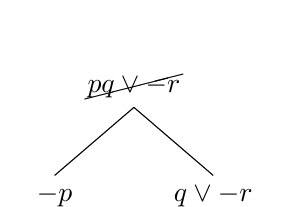
\begin{tikzpicture}[level distance=40pt, sibling distance=30pt] 
\tikzset{every tree node/.style={align=center,anchor=north}}
\Tree [.$\cancel{p\imp q\lor -r}$ 
		[.$-p$ ] 
		[.$q\lor -r$ ]
]
\end{tikzpicture}
\end{align}

given that a conditional of the form $P\imp Q$ is true whenever $P$ is false or
$Q$ is true. When we are done with decomposing a formula we cross it out to
avoid confusion.

In the next step, we decompose the disjunction on the right branch, how to
decompose a disjunction should not be hard to see:


\begin{align}
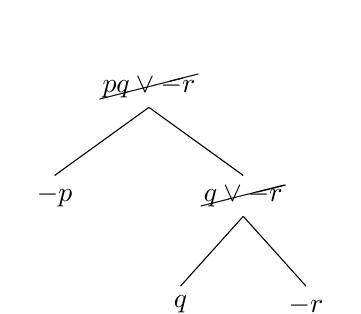
\begin{tikzpicture}[level distance=40pt, sibling distance=30pt] 
\tikzset{every tree node/.style={align=center,anchor=north}}
\Tree [.$\cancel{p\imp q\lor -r}$ 
		[.$-p$ ] 
		[.$\cancel{q\lor -r}$ 
			[.$q$ ] [.$-r$ ] ]		
		]
]
\end{tikzpicture}
\end{align}

We stop when we have only propositional symbols (or variables) and their
negations on the leaves of the tree. We check all the paths in the tree for
contradictions. A path has contradiction if there is both $P$ and $-P$ on it for
some formula $P$. We mark a path with a contradiction with
`$\times$' and those without contradiction with `$\surd$'. In our present case
no path has contradictions:

\begin{align}\label{ftree}
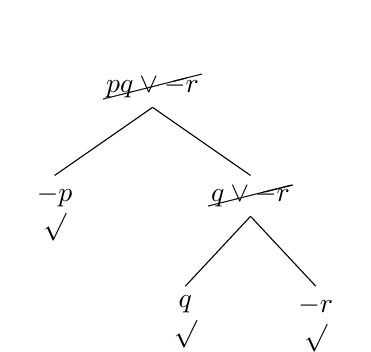
\begin{tikzpicture}[level distance=40pt, sibling distance=30pt] 
\tikzset{every tree node/.style={align=center,anchor=north}}
\Tree [.$\cancel{p\imp q\lor -r}$ 
		[.$-p$\\$\surd$ ] 
		[.$\cancel{q\lor -r}$ 
			[.$q$\\$\surd$ ] [.$-r$\\$\surd$ ] ]		
		]
]
\end{tikzpicture}
\end{align}

The tree in \xref{ftree} contains all the information present in the truth-table
\xref{ttex} in a more concise way. Each non-contradictory path corresponds to a
set of rows in the truth-table. For instance the left most path which has $-p$
stands for all the four rows in the table which has a 0 for $p$, and shows that
in all these rows the main formula has the truth-value 1.

\qed
\end{uexample}

\begin{uexample}
Now let us have a more complicated example:

\[
(-p\lor q \imp r) \land (-q \imp s)
\]

For a conjunction to hold both conjuncts must hold, licensing the following
decomposition:

\begin{align}
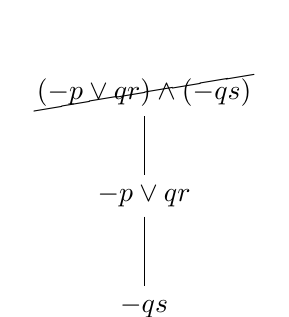
\begin{tikzpicture}[level distance=40pt, sibling distance=30pt] 
\tikzset{every tree node/.style={align=center,anchor=north}}
\Tree [.$\cancel{(-p\lor q\imp r)\land (-q\imp s)}$ 
		[.$-p\lor q\imp r$ $-q\imp s$ ] ]
\end{tikzpicture}
\end{align}

We do not branch as both conjuncts should hold at the same time, they are not
alternatives as was the case in disjunction and conditional.

We always continue decomposing from the left- and topmost decomposable formula.
In the present case we have a conditional:

\begin{align}
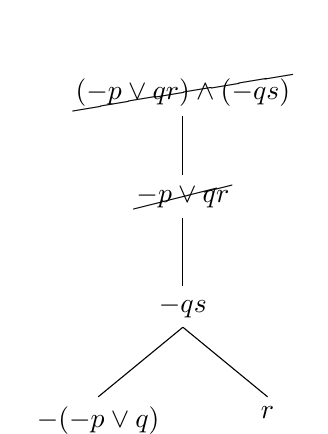
\begin{tikzpicture}[level distance=40pt, sibling distance=30pt] 
\tikzset{every tree node/.style={align=center,anchor=north}}
\Tree [.$\cancel{(-p\lor q\imp r)\land (-q\imp s)}$ 
		[.$\cancel{-p\lor q\imp r}$ 
			[.$-q\imp s$ 
				[.$-(-p\lor q)$ ]	
				[.$r$ ]
			] 
		]
	  ]
\end{tikzpicture}
\end{align}

The left- and topmost decomposable formula is $-q\imp s$, we continue from
there. This decomposition leads to branching with $--q$ and $s$. We will always
cancel double negations without showing it as a separate step. Therefore, the
branches will be $q$ and $s$. 

At this point we need to be careful in applying the branching resulting from
this decomposition to all the nodes that are reachable from the decomposed
formula by going only down. The result is: 

\begin{align}
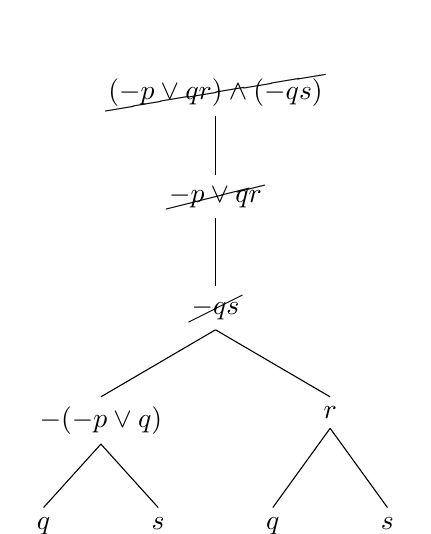
\begin{tikzpicture}[level distance=40pt, sibling distance=30pt] 
\tikzset{every tree node/.style={align=center,anchor=north}}
\Tree [.$\cancel{(-p\lor q\imp r)\land (-q\imp s)}$ 
		[.$\cancel{-p\lor q\imp r}$ 
			[.$\cancel{-q\imp s}$ 
				[.$-(-p\lor q)$ 
					[.$q$ ] [.$s$ ]
				]	
				[.$r$ $q$ $s$ 
				]
			] 
		]
	  ]
\end{tikzpicture}
\end{align}

One more formula is left to be decomposed, which is the negation of a
disjunction. A disjunction is false only when both disjuncts are false.
Therefore decomposition proceeds as follows:

\begin{align}
\begin{tikzpicture}[level distance=40pt, sibling distance=30pt] 
\tikzset{every tree node/.style={align=center,anchor=north}}
\Tree [.$\cancel{(-p\lor q\imp r)\land (-q\imp s)}$ 
		[.$\cancel{-p\lor q\imp r}$ 
			[.$\cancel{-q\imp s}$ 
				[.$\cancel{-(-p\lor q)}$ 
					[.$q$ 
					[.$p$ $-q$\\$\times$ ]	
					] 
					[.$s$ 
					[.$p$ $-q$\\$\surd$ ]	
					]
				]	
				[.$r$ $q$\\$\surd$ $s$\\$\surd$ 
				]
			] 
		]
	  ]
\end{tikzpicture}
\end{align}

\qed
\end{uexample}


\item Now it is time to list decomposition rules for each connective and
and their negation:
\newpage
\item[]{\bf Truth-tree construction rules:}

\begin{align}
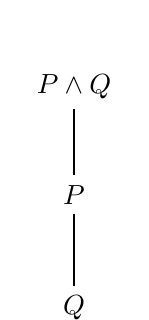
\begin{tikzpicture}[level distance=40pt, sibling distance=30pt] 
\tikzset{every tree node/.style={align=center,anchor=north}}
\Tree [.$P\land Q$ [.$P$ $Q$ ] ]
\end{tikzpicture}
\quad\quad\quad
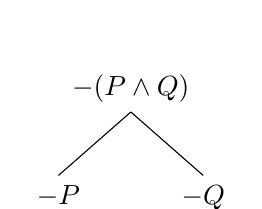
\begin{tikzpicture}[level distance=40pt, sibling distance=30pt] 
\tikzset{every tree node/.style={align=center,anchor=north}}
\Tree [.$-(P\land Q)$ $-P$ $-Q$ ]
\end{tikzpicture}
\end{align}

\begin{align}
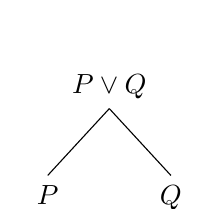
\begin{tikzpicture}[level distance=40pt, sibling distance=30pt] 
\tikzset{every tree node/.style={align=center,anchor=north}}
\Tree [.$P\lor Q$ $P$ $Q$  ]
\end{tikzpicture}
\quad\quad\quad
\begin{tikzpicture}[level distance=40pt, sibling distance=30pt] 
\tikzset{every tree node/.style={align=center,anchor=north}}
\Tree [.$-(P\lor Q)$ [.$-P$ $-Q$ ] ]
\end{tikzpicture}
\end{align}

\begin{align}
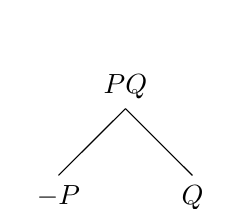
\begin{tikzpicture}[level distance=40pt, sibling distance=30pt] 
\tikzset{every tree node/.style={align=center,anchor=north}}
\Tree [.$P\imp Q$ $-P$ $Q$  ]
\end{tikzpicture}
\quad\quad\quad
\begin{tikzpicture}[level distance=40pt, sibling distance=30pt] 
\tikzset{every tree node/.style={align=center,anchor=north}}
\Tree [.$-(P\imp Q)$ [.$P$ $-Q$ ] ]
\end{tikzpicture}
\end{align}

\begin{align}
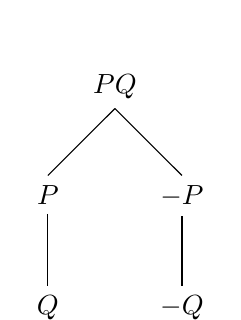
\begin{tikzpicture}[level distance=40pt, sibling distance=30pt] 
\tikzset{every tree node/.style={align=center,anchor=north}}
\Tree [.$P\bicond Q$ [.$P$  $Q$ ] [.$-P$  $-Q$ ]]
\end{tikzpicture}
\quad\quad\quad
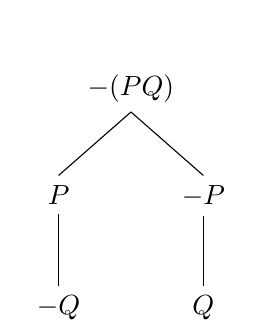
\begin{tikzpicture}[level distance=40pt, sibling distance=30pt] 
\tikzset{every tree node/.style={align=center,anchor=north}}
\Tree [.$-(P\bicond Q)$ [.$P$ $-Q$ ] [.$-P$ $Q$ ] ]
\end{tikzpicture}
\end{align}

\hrulefill
\begin{uexercise}\label{treecons}

Construct truth-trees for the following formulas:

\begin{enumerate}
\item $(p\imp q) \imp (p\imp q\lor r)$
\item $(p\imp q) \imp (p\imp q\land r)$
\item $(p\land s) \bicond (q \lor r)$
\item $((p\imp q) \imp s)\land (p\imp (q\imp s))$
\item $p\land (-q\lor -p)$
\item $((p\imp -q) \imp -p) \imp q$
\item $(p\imp q) \imp (-p \imp -q)$
\item $(p\imp q) \imp (-q \imp -p)$
\item $((p\imp q)\imp p) \imp p$
\item $(p\lor q) \imp (p\imp q)$
\item $(p\imp q) \land (q\imp r) \land (r\imp p)$
\item $(p\imp q) \land (q\imp r) \land (r\imp p)$
\item $-(-(-p\land -q)\land -p)\bicond -(q\lor -p)$

\end{enumerate}
\qed
\end{uexercise}
\hrulefill

\hrulefill
\begin{uexercise}\label{treeconsfol}
Inspecting the trees for the previous question, do you find it easy to discover
the valuations that make the formula false? Any useful strategy for this task?

\qed
\end{uexercise}
\hrulefill


\hrulefill
\begin{uexercise}\label{treeconsfol}
You are given that Mary, a graduate student, is such that:

\begin{quote}\small
If she studies, she  gets good grades.\\
If she doesn't study, she enjoys life.\\
If she doesn't get good grades, she doesn't enjoy life.
\end{quote}

Symbolize these statements in propositional logic and construct a truth-tree to
answer the following questions:

\begin{enumerate}
\item Does she enjoy life?
\item Does she get good grades?
\end{enumerate}

\qed
\end{uexercise}
\hrulefill

\hrulefill
\begin{uexercise}\label{treeconsfol}
We have the following information:

\begin{quote}\small
If samples are contaminated, then there is leakage in the reactor or there is
non-consumed fuel.\\ 
All the fuel is consumed.\\
There is no leakage in the reactor or the detector is malfunctioning.\\
The detector is functioning properly.

\end{quote}

Someone asserts that samples are contaminated. Do we need to believe? Motivate
your answer by constructing a truth-tree.

\qed
\end{uexercise}
\hrulefill
\end{itemize}


\section{Validity, contradictoriness, consistency}

\ezimeti{
\item A formula $P$ is \uterm{valid} if and only if it comes out true with every
valuation.

\item[] We designate the validity of $P$ by:

$$
\models P
$$

\item[] Valid formulas of propositional logic are also called
\uterm{tautologous}. 

\item[] Some examples:

\begin{align*}
&\models p\lor -p \\ &\models p\imp(q\imp p) 
\end{align*}


\item A formula $P$ is \uterm{contradictory}, designated $\not\models P$, if and only if it comes out
false in every valuation.

\hrulefill
\begin{uexercise}
Can you think of a general method of testing whether a given formula is valid,
contradictory, or consistent?
\end{uexercise}
\hrulefill
}

\section{Implication, equivalence and substitution}
\ezimeti{

\item A formula $P$ \uterm{implies} $Q$, designated $P\models Q$, if and only if
$\models P\imp Q$.


\item Two formulas $P$ and $Q$ are \uterm{equivalent}, designated $P\equiv Q$, if and only if
$\models P\leftrightarrow Q$.

\item Given a formula $R$, $R \equiv R_{[P/Q]}$ iff
$P\equiv Q$, where $R_{[P/Q]}$ means the formula formed by substituting $P$ for
each occurrence of $Q$ in $R$. 

\hrulefill
\begin{uexercise}
Given `$p \imp q$', state which of the following imply or are implied by it:
\setlength{\arraycolsep}{1.4em}
$$
\begin{array}{cccc}
-p & q & -p \lor q & q \land r  \\
&  p \imp q \lor r &  p \lor r \imp q  & \\   
p \imp q \land r  & (p\imp q) \lor r &  -q\imp -p &  p \land r \imp q \\
\end{array}
$$
\end{uexercise}
\hrulefill
}

\section{Natural deduction}

Natural deduction is a method for \uterm{deriving} a formula $Q$ from (possibly
empty) set of formulas $\crbr{P_1,P_2,\ldots,P_n}$, called \uterm{premisses},
such that $Q$ is true in case all the premisses are jointly true. The relation
of derivability is designated as:


$$P_1,P_2,\ldots,P_n \vdash Q$$

and,

$$P_1,P_2,\ldots,P_n \vdash Q\quad \text{ iff }\quad P_1\land P_2\land \ldots\land P_n
\models Q$$

The method of natural deduction  involves a set of \uterm{inference rules} and
\uterm{proof techniques}.


\subsection{Inference rules}

\begin{itemize}
\item[]{ Simplification:}
$$
\begin{array}{c}
P\land Q\\ \hline
P
\end{array}
\quad
\quad
\quad
\begin{array}{c}
P\land Q\\ \hline
Q
\end{array}
$$

\item[]{Adjunction:}

$$
\begin{array}{c}
P \\
Q \\ \hline
P \land Q
\end{array}
\quad
\quad
\quad
\begin{array}{c}
P \\
Q \\ \hline
Q \land P
\end{array}
$$

\item[]{Addition:}

$$
\begin{array}{c}
P \\ \hline

P \lor Q \\
\end{array}
\quad
\quad
\quad
\begin{array}{c}
Q \\ \hline
P \lor Q
\end{array}
$$

\item[]{Modus ponens (MP):}

$$
\begin{array}{l}
P \imp Q \\ 
P \\ \hline
Q \\ 
\end{array}
$$

\item[]{Modus tollens (MT):}

$$
\begin{array}{l}
P \imp Q \\ 
-Q \\ \hline
-P \\ 
\end{array}
$$
\item[]{Modus tollendo ponens (MTP):}

$$
\begin{array}{l}
P \lor Q \\
-P \\ \hline
Q \\
\end{array}
\quad
\quad
\quad
\begin{array}{l}
P \lor Q \\
-Q \\ \hline
P \\
\end{array}
$$

\item[]{Double negation:}

$$
\begin{array}{c}
--P \\ \hline 
P \\ 
\end{array}
\quad
\quad
\quad
\begin{array}{c}
P \\ \hline 
--P \\ 
\end{array}
$$

\item[]{Repetition:}

$$
\begin{array}{c}
P \\ \hline
P \\ 
\end{array}
$$
\end{itemize}



\subsection{Proof techniques}

\subsubsection{Direct proof}

Let's illustrate how a direct proof works over an example,

$$p\land q \vdash q\land p$$

We start by designating our target -- the formula we aim to derive:


In proofs we can pick and add any of our premisses at any point, if we
believe it will be useful. Here we do that, and add our only premiss.

\begin{logicproof}{2}
	\sform{q\land p} & \\
	\form{p\land q} &\label{prem} Prem.
\end{logicproof}

Next we observe that we can apply one of our rules, simplification, to the premiss twice,
obtaining $p$ and $q$. In the ideal case we write the justification of each
step. 

\begin{logicproof}{2}
	\sform{q\land p} & \\
	\form{p\land q} & Prem.\\		
	\form{p} & \ref{prem} Simp.\\		
	\form{q} & \ref{prem} SSimp.
\end{logicproof}


Next we use another rule, adjunction, to form the desired formula

\begin{logicproof}{2}
	\sform{q\land p} & \\
	\form{p\land q} & Prem.\\		
	\form{p} & \ref{prem} Simp.\\		
	\form{q} & \ref{prem} Simp.\\		
	\form{q\land p} & Adj.
\end{logicproof}


In a direct proof, when we obtain the formula we wanted to derive, we
``box'' the proof, and cancel the initial $Show$.

\begin{logicproof}{3}
	\cform{q\land p} & \\
	\begin{subproof}
	\form{p\land q} & Prem.\\		
	\form{p} & \ref{prem}\label{s1} Simp.\\		
	\form{q} & \ref{prem}\label{s2}  Simp.\\		
	\form{q\land p} & \ref{s1}, \ref{s2} Adj.
	\end{subproof}
\end{logicproof}

Although direct proof is conceptually simple, it is seldom adequate on
its own.


\subsubsection{Conditional proof}

When the target formula is a conditional, we assume the antecdent and
show that the consequent is derviable under this assumption. Take,  

\begin{align}
-q\imp -r,\quad p \imp r\;\vdash\; p\imp q
\end{align}




Again we start with a \textit{Show} line. 

\begin{logicproof}{3}
	\sform{p\imp q} &
\end{logicproof}

In a conditional proof, we start with assuming the antecedent, $p$ in
this case:

\begin{logicproof}{3}
	\sform{p\imp q} & \\
	\form{p} & \label{bass}Asmp.		
\end{logicproof}

The aim is to derive the consequent $q$. In this task, in addition to
the premisses, we are allowed to make use of the assumption $p$.From here on we
proceed as in a direct proof of $q$, namely applying the available rules to the
formulas available. It is crucial to observe that we cannot apply MP to $p\imp
q$ and $p$. Any formula that has an uncancelled \textit{Show} is UNavailable in a
proof. In order to proceed,  we take a premiss that we can feed into the MP rule
together with $p$ and obtain $r$.


\begin{logicproof}{3}
	\sform{p\imp q} & \\
	\form{p} & \label{bass}Asmp.	\\	
	\form{p\imp r} & \label{bp2} Prem.\\
	\form{r} & \ref{bass}, \ref{bp2} \label{br}  MP
\end{logicproof}

The rest of the proof proceeds in a similar fashion, eventually
obtaining $q$, boxing the proof and cancelling the \textit{Show}.

\begin{logicproof}{3}
	\cform{p\imp q} & \\
	\begin{subproof}
	\form{p} & \label{bass}Asmp.	\\	
	\form{p\imp r} & \label{bp2} Prem.\\		
	\form{r} & \ref{bass}, \ref{bp2} \label{br}  MP\\
	\form{--r} & \ref{br}\label{b-r} DN\\
	\form{-q\imp -r} & \label{bp1} Prem.\\
	\form{--q} & \ref{b-r}, \ref{bp1}\label{b--q} MT\\
	\form{q} & \ref{b--q} DN
	\end{subproof}
\end{logicproof}

Now we turn to an example that calls for nested \textit{Show}s. Take,

\begin{align}
p\imp(q\imp r),\quad p\imp(r\imp s)\; \vdash\; p\imp(q\imp s)
\end{align}

We start our conditional proof by assuming $p$:

\begin{logicproof}{3}
	\sform{p\imp (q\imp s)} & \\
	\form{p} & \label{cass1}Asmp.
\end{logicproof}

At this point we have a new goal, proving $q\imp s$. If we can do that,
then we can conclude that assuming $p$ yields $q\imp s$, achieving our initial
goal.

\begin{logicproof}{3}
	\cform{p\imp (q\imp s)} & \\
	\form{p} & \label{cass1}Asmp.	\\	
	\sform{(q\imp s)} & \\
\end{logicproof}

In our \uterm{subproof} we proceed as in a conditional proof, assuming
$q$ and trying to obtain $s$: 


\begin{logicproof}{3}
	\sform{p\imp (q\imp s)} & \\
	\form{p} & \label{cass1}Asmp.	\\	
	\sform{(q\imp s)} & \\
	\form{q} & \label{cass2}Asmp.	\\
\end{logicproof}

Once we obtain $s$ we box its proof and cancel the \textit{Show}
preceeding our interim goal $q\imp s$, 

\begin{logicproof}{3}
	\sform{p\imp (q\imp s)} & \\
	\form{p} & \label{cass1}Asmp.	\\	
	\cform{(q\imp s)} & \\
	\begin{subproof}	
	\form{q} & \label{cass2}Asmp.	\\
	\form{p\imp(q\imp r)} & Prem. \label{cp1}\\ 
	\form{q\imp r} & \ref{cass1}, \ref{cp1} MP\label{cqr}\\
	\form{r} & \ref{cass2}, \ref{cqr} MP\label{cr}\\
	\form{p\imp (r\imp s)} & \label{cp2} Prem.\\		
	\form{r\imp s} & \ref{cass1}, \ref{cp2}  MP\label{crs}\\		
	\form{s} & \ref{cr}, \ref{crs}  MP		
	\end{subproof}
\end{logicproof}

Our initial aim was to see whether we can obtain $q\imp s$ under the
assumption $p$ (and of course our premisses). Any formula that is preceeded by a
cancelled \cform is available for use in the unboxed parts of our proof. Given
that, we see that we derived $q\imp s$ on the assumption $p$. We box the proof
and cancel our top-most \emph{Show}:

\begin{logicproof}{3}
	\cform{p\imp (q\imp s)} & \\
	\begin{subproof}
	\form{p} & \label{cass1}Asmp.	\\	
	\cform{(q\imp s)} & \\
	\begin{subproof}	
	\form{q} & \label{cass2}Asmp.	\\
	\form{p\imp(q\imp r)} & Prem. \label{cp1}\\ 
	\form{q\imp r} & \ref{cass1}, \ref{cp1} MP\label{cqr}\\
	\form{r} & \ref{cass2}, \ref{cqr} MP\label{cr}\\
	\form{p\imp (r\imp s)} & \label{cp2} Prem.\\		
	\form{r\imp s} & \ref{cass1}, \ref{cp2}  MP\label{crs}\\		
	\form{s} & \ref{cr}, \ref{crs}  MP		
	\end{subproof}
	\end{subproof}
\end{logicproof}

\subsubsection{Indirect proof}

An indirect proof starts with assuming the opposite (denial) of what is being
tried to be proved. If this assumption leads to a contradiction -- having both
$P$ and $-P$ for some formula $P$, we conclude that the formula we denied in the
beginning holds. This technique is sometimes called `proof by contradiction' or
\emph{reductio ad absurdum}.

\begin{uexample}
Prove \ref{ind1} by natural deduction.
\begin{align}\label{ind1}
-p\imp q,\quad p\imp q\; \vdash\; q
\end{align}

We start by denying our target $q$:

\begin{logicproof}{2}
\sform{q} &\\
\form{-q} & Asmp. \label{eass}
\end{logicproof}

From here on our aim is to derive a contradiction. \emph{Any} formula $P$ such
that we have both $P$ and $-P$. We achieve this aim as follows:

\begin{logicproof}{2}
\sform{q} &\\
\form{-q} & Asmp. \label{eass}\\
\form{p\imp q} & Prem.\label{ep1}\\
\form{-p} & \ref{eass}, \ref{ep1} TP\label{e-p}\\
\form{-p\imp q} & Prem.\label{ep2}\\ 
\form{q} & \ref{e-p}, \ref{ep2} MP
\end{logicproof}

Our assumption $-q$ has allowed us to derive $q$, resulting in a contradiction.
We can now conclude that the assumption $-q$ is unatainable, and therefore $q$
must hold. This completes the proof. We box and cancel as usual. 

\begin{logicproof}{2}
\cform{q} &\\
\begin{subproof}
\form{-q} & Asmp. \label{eass}\\
\form{p\imp q} & Prem.\label{ep1}\\
\form{-p} & \ref{eass}, \ref{ep1} MP\label{e-p}\\
\form{-p\imp q} & Prem.\label{ep2}\\ 
\form{q} & \ref{e-p}, \ref{ep2} MP
\end{subproof}
\end{logicproof}

\qed
\end{uexample}


\begin{uexample}
Take the following argument:

\begin{quote}

Harry is the murderer, only if he was at the apartment around 10pm. The police will
find a fingerprint, provided that he was at the apartment around 10pm. It
is not the case that if he forgot to wear a glove, the police will find a
fingerprint. Therefore, Harry is not the murderer.

\end{quote}

Given the symbolization,

\begin{itemize}
\item[] $m$: Harry is the murderer;
\item[] $r$: Harry was at the apartment around 10pm;
\item[] $p$: The police will find a fingerprint;
\item[] $t$: Harry forgot to wear a glove, 
\end{itemize}

the argument will be:\footnote{Note that `$p$ only if $q$' is $p\imp q$, while
`$p$ provided that $q$' is $q\imp p$. }

\begin{align}
m\imp r,\quad r\imp p\quad -(t\imp p)\;\vdash\; -m
\end{align}


We proceed with an indirect proof:

\begin{logicproof}{2}
\sform{-m} & \\
\form{--m} & Asmp.\label{dass}\\
\form{m}  & \ref{dass} DN\label{dm}
\end{logicproof}

The same proof could be started as,

\begin{logicproof}{2}
\sform{-m} & \\
\form{m}  & Asmp.\label{dass}\label{dm}
\end{logicproof}
leaving the application of DN implicit. Now, the aim is to derive a
contradiction. The most basic strategy is to derive some formula that
contradicts what we already have in the proof and unused premisses, if there are
any. Let's attempt to derive $t\imp p$ via a conditional subproof:  

\begin{logicproof}{2}
\sform{-m} & \\
\form{m}  & Asmp.\label{dm}\\
\cform{t\imp p} &\\
\begin{subproof}
\form{t} & \label{dass}\\
\form{m\imp r} & Prem.\label{dp1}\\
\form{r} & \ref{dm}, \ref{dp1} MP\label{dr}\\
\form{r\imp p} & Prem.\label{dp2}\\
\form{p} & \ref{dr}, \ref{dp2} MP\label{dr}
\end{subproof}
\end{logicproof}

Having proved $t\imp p$, we arrived at a contradiction, namely with the premiss
$-(t\imp p)$:

\begin{logicproof}{2}
\sform{-m} & \\
\form{m}  & Asmp.\label{dm}\\
\form{-(t\imp p)} & Prem.\label{dp3}\\
\cform{t\imp p} &\\
\begin{subproof}
\form{t} & \label{dass}\\
\form{m\imp r} & Prem.\label{dp1}\\
\form{r} & \ref{dm}, \ref{dp1} MP\label{dr}\\
\form{r\imp p} & Prem.\label{dp2}\\
\form{p} & \ref{dr}, \ref{dp2} MP\label{dr}
\end{subproof}
\end{logicproof}
which completes our proof as:

\begin{logicproof}{2}
\cform{-m} & \\
\begin{subproof}
\form{m}  & Asmp.\label{dm}\\
\form{-(t\imp p)} & Prem.\label{dp3}\\
\cform{t\imp p} &\\
\begin{subproof}
\form{t} & \label{dass}\\
\form{m\imp r} & Prem.\label{dp1}\\
\form{r} & \ref{dm}, \ref{dp1} MP\label{dr}\\
\form{r\imp p} & Prem.\label{dp2}\\
\form{p} & \ref{dr}, \ref{dp2} MP\label{dr}
\end{subproof}
\end{subproof}
\end{logicproof}

\qed
\end{uexample}

\section*{Self study} Except natural deduction, you can review what we have
covered in propositional logic from \cite{parteeetal90}, Chapter 6, up to
Section 6.5. Please note some terminological differences: they use ``statement
logic'' for ``propositional logic'', ``logical consequence'' for
``implication'', ``disjunction'' for ``alternation'', ``contingent'' for
``consistent'', and so on.

Please do not try to memorize Table 6.2. The caption of the table, ``Laws of
statement logic'' is misleading. These are not laws, they are just valid
formulas, which are on an equal status with any other valid formula of propositional
logic. Try to see and work out why they are valid, and that's it for now.

As for the inductive definitions of the well-formed expressions of $L_0$ and
their top-down analysis and bottom-up generation (Section \ref{induc} of the
notes), they can be reviewed from
the notes. If you do not fully understand them at the moment, don't worry. Give
priority to the logic part. 


\renewcommand{\bibsep}{0pt}
\renewcommand{\bibfont}{\small}
\bibliography{ozge}
\bibliographystyle{natgig}
\end{document}

\item We will use capital symbols $P,Q,R,S$ and their subscripted forms as variables standing for formulas.  
\item For any formulas $P$, $Q \in L_0$:
\begin{align*}
(P \land Q) &\text{ is true, if and only if both } P \text{ and } Q \text{ are 
true.}\\
(P \lor Q) &\text{ is true, if and only if at least one of } P \text{ and } Q \text{
is true.}\\
(-P) &\text{ is true, if and only if } P \text{ is false.}
\end{align*}

\item Conjunction and alternation enjoy certain properties familiar from set
union and intersection:
\begin{align*}
(P\land P) &= P\\
(P\land Q) &= (Q\land P)\\
((P\land Q)\land R) &= (P\land (Q\land R))
\end{align*}
and likewise for alternation.
\item Observe that the equalities we list above are on the basis of truth
values. There is no way the two equated sentences can differ in their truth
value.
